%!TEX root = ../report.tex

\chapter{Map Stitching with the Hough Transform}
\label{chapter:hough}
Why hough based?
Alternatives?

[what is map stitching, why is it necessary again?]

Stefano Carpin presented a novel map stitching approach based on the Hough Transform in \cite{carpin2002merging}. It is an extention of the Hough transform which Censi et~al.\ introduced as the \emph{Hough spectrum} \cite{censi2005scan}. Censi et~al.\ used the hough spectrum for a novel scan matcher. 

Remember from the SLAM section (\ref{state}) that aligning two maps takes two parameters: the rotation angle $\theta$ and translation vector $t = [x, y]^T$. The Hough spectrum is used for finding the rotation $\theta$ between a scan and reference map. The implementations of Carpin and Censi et~al.\ diverge in their method of finding the translation vector $t$ between two scans. 

The Hough-based map stitching works with the assumption of an indoor environment. It is a global method, and does not take into consideration any prior knowledge about the relative alignment of both pieces of the map.

This chapter is setup as follows. First, we'll look at what the Hough transform and Hough spectrum are. Then, we'll take a look at how the best matching rotation $\hat\theta$ is found, and finally we'll examine translation $t$ further. This chapter concludes with an elaborate example.

\section{Hough transform}
The Hough transform is in origin a line detection technique, patented by Paul Hough in 1962\cite{hough1962method}. An improved version, which is presented here, was introduced by Duda and Hart\cite{duda1972use}. The Hough transform is also extended to detect circles, ellipsis and parabolas, and also arbitrary 2D shapes\cite{ballard1981generalizing}.

The Hough transform detects lines in the following manner. A line in Cartesian $(x, y)$ space can be defined by it's angle ($\theta$) and distance from the origin $\rho$:

\begin{equation}
\label{eq:line}
x\cos \theta + y\sin \theta = \rho
\end{equation}

Every point in $(x,y)$ space lies on infinitely many lines satisfying equation~\ref{eq:line}. Every angle $\theta$ has a single accompanying distance from the origin $\rho$. Thus, a point in $(x,y)$ space can be represented in the \emph{Hough domain} $(\theta, \rho)$ as a curve. The locations where many curves intersect in the Hough domain correspond to the lines in the original image; remember that lines correspond to points in the Hough domain. 

Finding the intersection of many curves in the continuous domain is computationally expensive. The discrete Hough transform mitigates this problem by discretizing the Hough domain into bins. Every point in the original image `votes' for each bin it belongs to in $(\theta, \rho)$ representation. The strongest lines stand out as bins with a high number of votes.

There are $n_\theta$ angle-bins, and $n_\rho$ distance bins in discrete Hough transform $\mathcal{HT}$. 

\begin{figure}[ht]
\centering
\subfigure[Two lines]{
	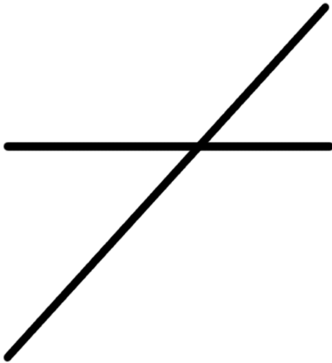
\includegraphics[width=0.4\textwidth]{images/stitching/lines.png}
	\label{fig:lines-original}
}
\subfigure[The Hough transform of \subref{fig:lines-original}]{
	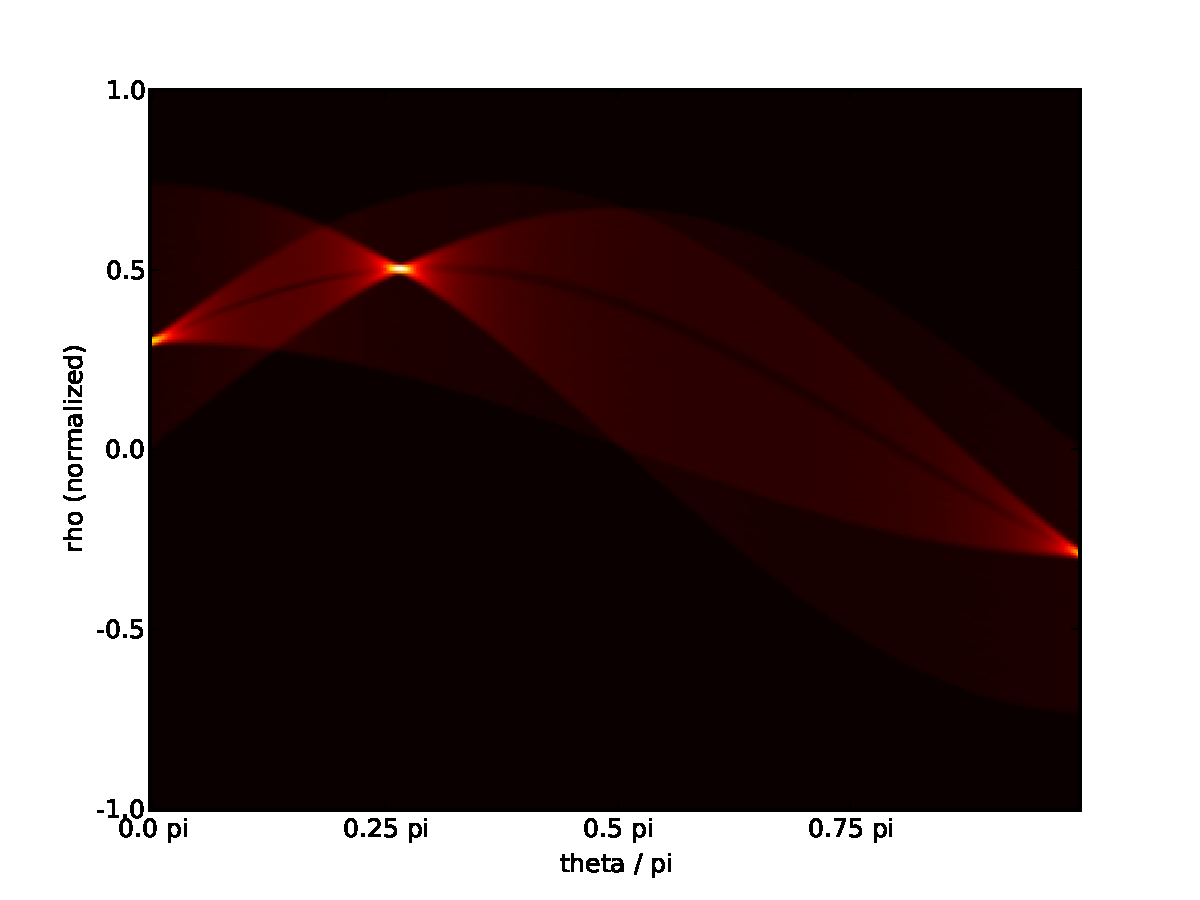
\includegraphics[width=0.55\textwidth]{images/stitching/lines-hough.pdf}
	\label{fig:lines-hough}
}
\caption{Example of the discrete Hough transform. Notice the two maxima in (b) which correspond to the two lines in (a). There seem to be three maxima (one at $0$, one at $\frac{\pi}{4}$ and one at $\pi$). However, the maxima at $0$ and $\pi$ are the same maximum; see section~\ref{sub:periodicity}.}
\label{fig:lines}
\end{figure}


\section{Hough spectrum}
The major contribution of Censi et~al.\ \cite{censi2005scan} is the introduction of the Hough spectrum. The Hough spectrum ($\cal HS$) is a measure for the direction of lines in an image. The discrete Hough transform finds the specific lines in the image, while the Hough spectrum finds the most pronounced \emph{directions} of lines in the image:

\begin{equation}
\mathcal{HS}(k) = \eta \sum_{i=1}^{n_\rho} \mathcal{HT} (i, k) ^ 2 \qquad \quad 1 \leq k \leq n_\theta
\end{equation}

$\eta$ is a normalization value to limit $\mathcal{HS}(k)$ to the domain $[0, 1]$.

As we've seen in the previous section, each bin in the discrete Hough transform ($\mathcal{HT} (i, k)$) contains the number of pixels that lie on a line defined by $(\theta_i, \rho_k)$. The hough spectrum is a measure for how strong the lines are on a specific angle. 

Thus, the Hough spectrum yields the highest value in the direction in which the most pronounced lines run. In an indoor environment, there will usually be two peaks, separated by a $90\degree$ angle, corresponding to grid-like structure most buildings are created (see figure~\ref{fig:rooms}). Incidentally, in a bee-hive, with hexagonal chambers, we would see 3 peaks each separated by $60\degree$  angles. See figure~\ref{fig:beehive}.

\begin{figure}[ht]
\centering
\subfigure[A stylistic map of some rooms]{
	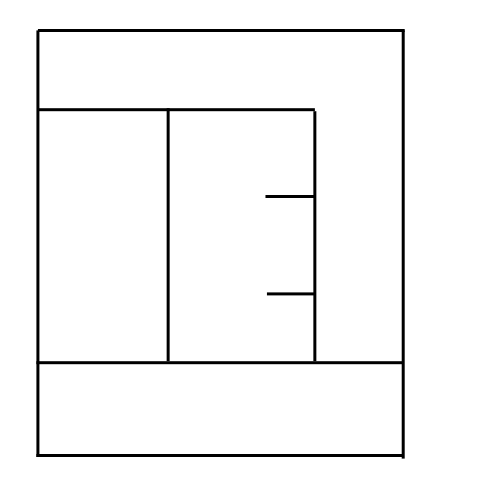
\includegraphics[width=0.4\textwidth]{images/stitching/rooms.png}
	\label{fig:rooms-original}
}
\subfigure[The Hough transform and Hough spectrum of \subref{fig:rooms-original}]{
	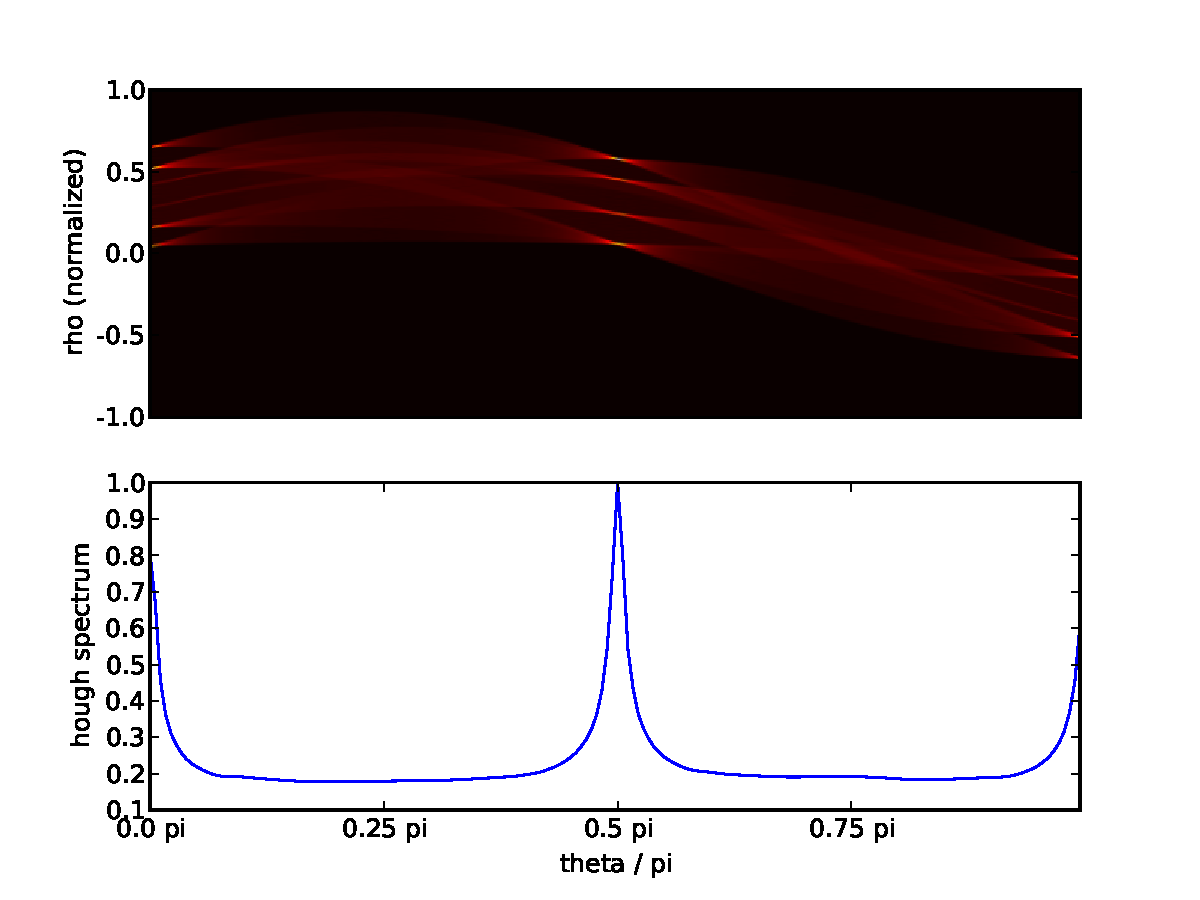
\includegraphics[width=0.55\textwidth]{images/stitching/rooms-hough.pdf}
	\label{fig:rooms-hough}
}
\caption{Example of a hough spectrum in a human-made environment.}
\label{fig:rooms}
\end{figure}

\begin{figure}[ht]
\centering
\subfigure[Hexagonal chambers]{
	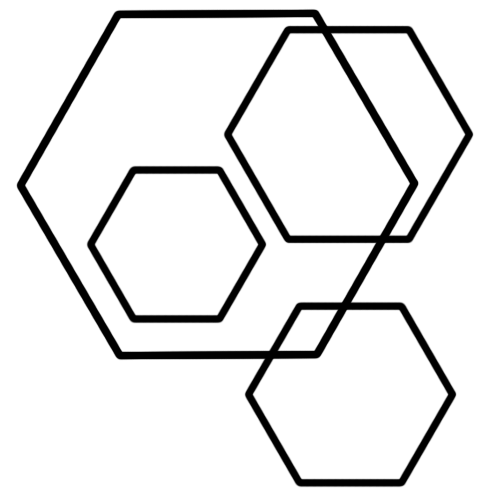
\includegraphics[width=0.4\textwidth]{images/stitching/beehive.png}
	\label{fig:beehive-original}
}
\subfigure[The Hough transform and Hough spectrum of \subref{fig:beehive-original}]{
	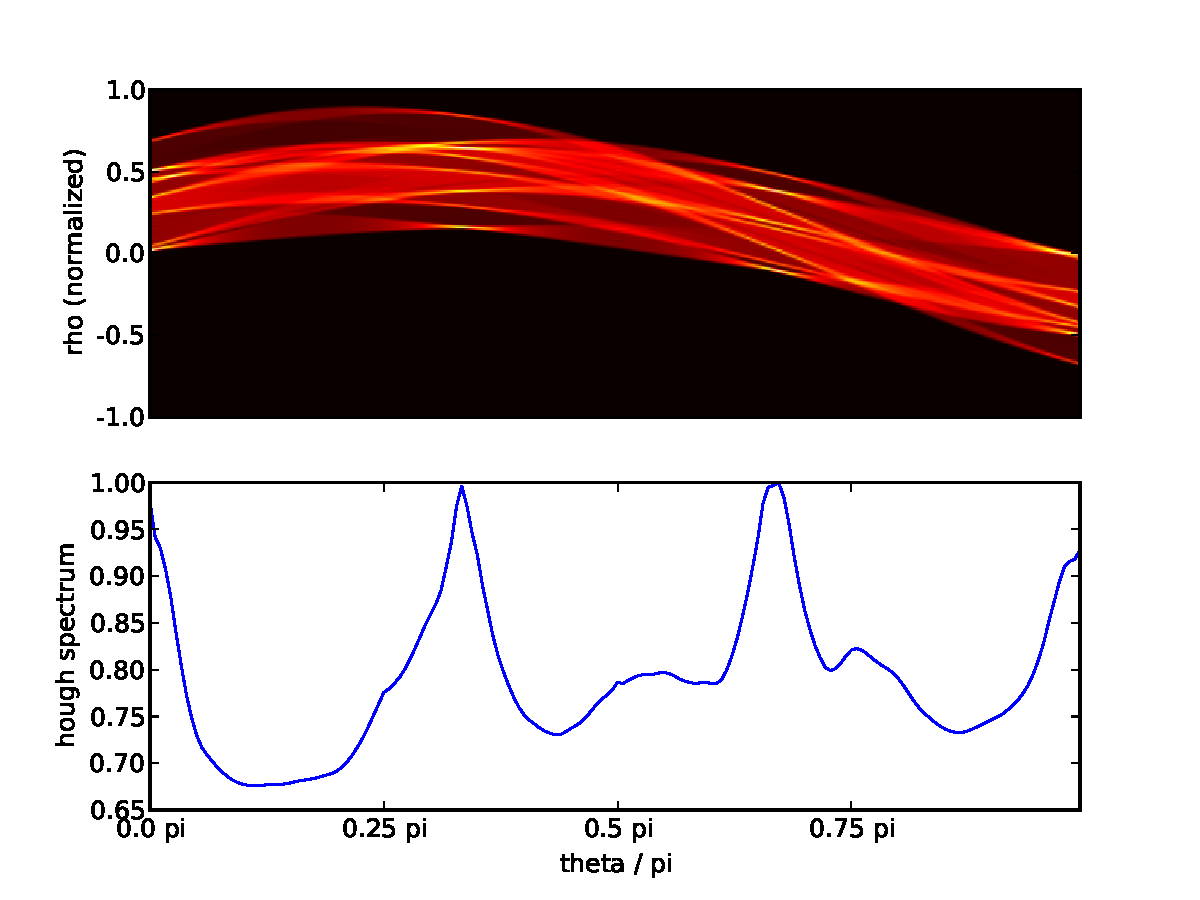
\includegraphics[width=0.55\textwidth]{images/stitching/beehive-lines.pdf}
	\label{fig:beehive-hough}
}
\caption{Example of the Hough spectrum in a hexagonal environment. Notice the three maxima in the Hough Spectrum.}
\label{fig:beehive}
\end{figure}

\section{Finding rotation $\theta$}
In the previous section we've seen how to calculate the Hough spectra $\mathcal{HS}_{M_1}$ and $\mathcal{HS}_{M_2}$ for maps $M_1$ and $M_2$. We will calculate the best rotation by performing a cross-correlation over the spectra. The cross-correlation of the two signals shows the similarity of the two spectra as one of them is shifted over the x-axis. The cross-correlation $\mathcal{CC}_{M_1,M_2}$ is calculated as follows:

\begin{equation}
\mathcal{CC}_{M_1,M_2}(k) = \sum_{i=1}^{n_\theta} \mathcal{HS}_{M_1}(i) \times \mathcal{HS}_{M_2}(i + k) \qquad 1 \leq k \leq n_\theta
\end{equation}

\begin{figure}[ht]
	\centering
	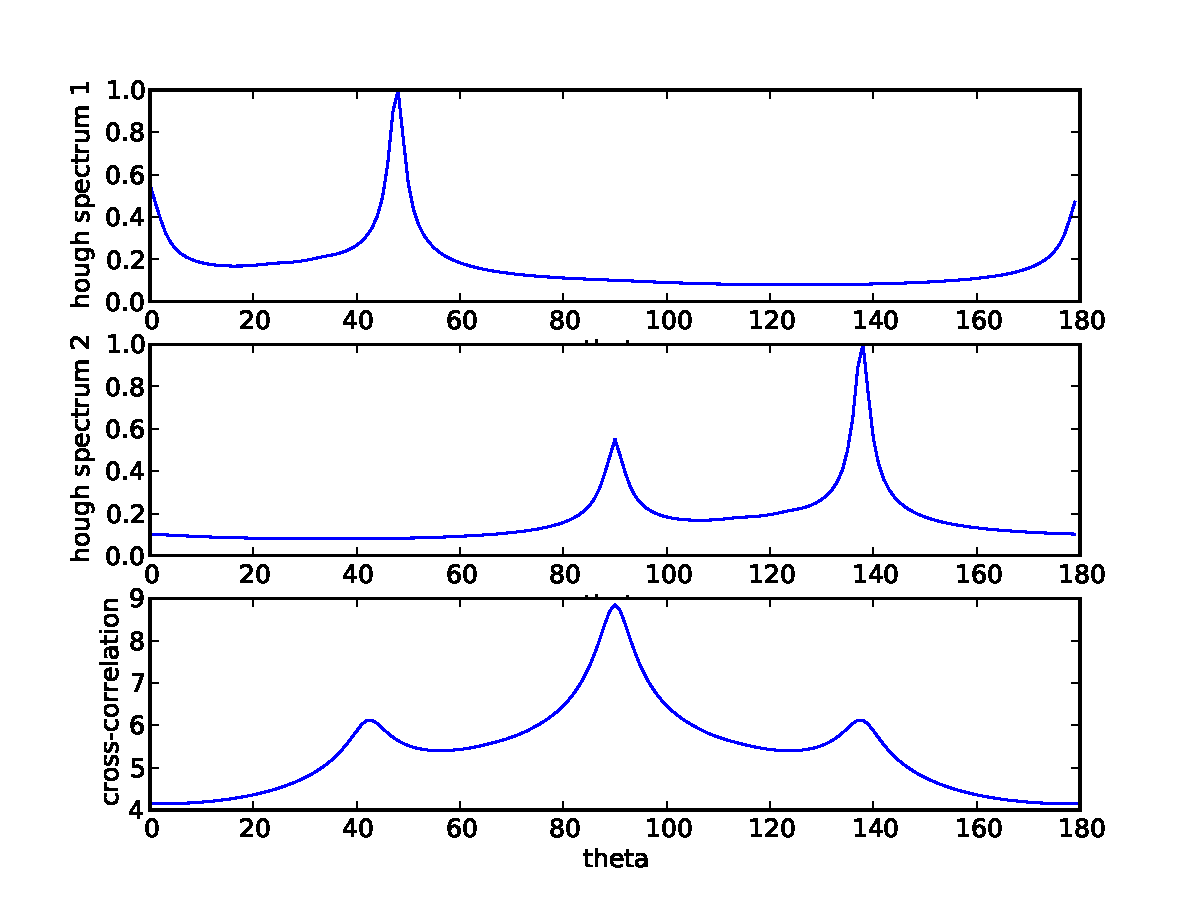
\includegraphics[width=\textwidth]{images/stitching/lines-cross-correlation.pdf}
	\caption{The top two plots are the hough spectra of image~\ref{fig:lines-original}. The image for the second hough spectrum was rotated $90\degree$ counter-clockwise. The cross-correlation shows that the most probable rotation is indeed $90\degree$, with smaller peaks for $45\degree$ and $135\degree$.}
	\label{fig:lines-cross-correlation}
\end{figure}

Notice that the spectra have a periodicity of $180\degree$ ($\pi$), and have similar peaks. However, the peaks are at different angles. The cross-correlation finds the optimal rotation; see figure~\ref{fig:lines-cross-correlation}.

\section{Periodicity of $\theta$}
\label{sub:periodicity}
Why are do the Hough spectra have a periodicity of $\pi$? The answer lies in the following equations:

\begin{eqnarray}
x\cos \theta + y\sin \theta &=& \rho \\
x\cos(\theta + \pi) + y\sin (\theta + \pi) &=& -\rho
\end{eqnarray}

Thus, the following equation holds: $\mathcal{HT}(\theta_\alpha, \rho_\alpha) = \mathcal{HT}(\theta_\alpha + \pi, -\rho_\alpha)$. In turn, the Hough spectrum of $\theta_\alpha$ and $\theta_\alpha + \pi$ are the same, because $\mathcal{HS}$ is summed over all $\rho$. 

Thus, the domain of $\theta$ only needs to be $[0, \pi \rangle$, whereafter it wraps back to itself. Prior work by Jankowska used the domain $[0, 2\pi\rangle$ \cite{jankowska2009hough}, which is thus superfluous.

One must take care when using this representation to remember the possible alternative hypothesis for $\theta$. Every candidate solution $\hat\theta$ found by the cross-correlation method has an additional solution $\hat\theta + \pi$!

\section{Finding translation $\hat t$}
In the previous section we found rotation candidates which align the maps according to the major wall-directions. To find the best match between two maps, we also need to find the optimal translation between them. Jankowska~\cite{jankowska2009hough} takes the same approach as Carpin~\cite{carpin2008merging}, which is a simplification of the method by Censi et~al.~\cite{censi2005scan}. We will discuss the more complex method later. 

The simplified method is to calculate an X-spectrum and Y-spectrum from the maps, and again perform cross-correlation on these. The X- and Y- spectra are calculated by summing the number of occupied pixels along one dimension; see equations~\ref{eq:x-spectrum} and \ref{eq:y-spectrum}. See figure~\ref{fig:x-y-spectra} for an example. The optimal translation is found by cross-correlating the x- and y-spectra from both maps.

\begin{eqnarray}
\label{eq:x-spectrum}
\textrm{X-spectrum}(x) = \sum_{y \in Y} \textrm{occupancyMap}(x, y) \\
\label{eq:y-spectrum}
\textrm{Y-spectrum}(y) = \sum_{x \in X} \textrm{occupancyMap}(x, y) 
\end{eqnarray}

\begin{figure}[ht]
	\centering
	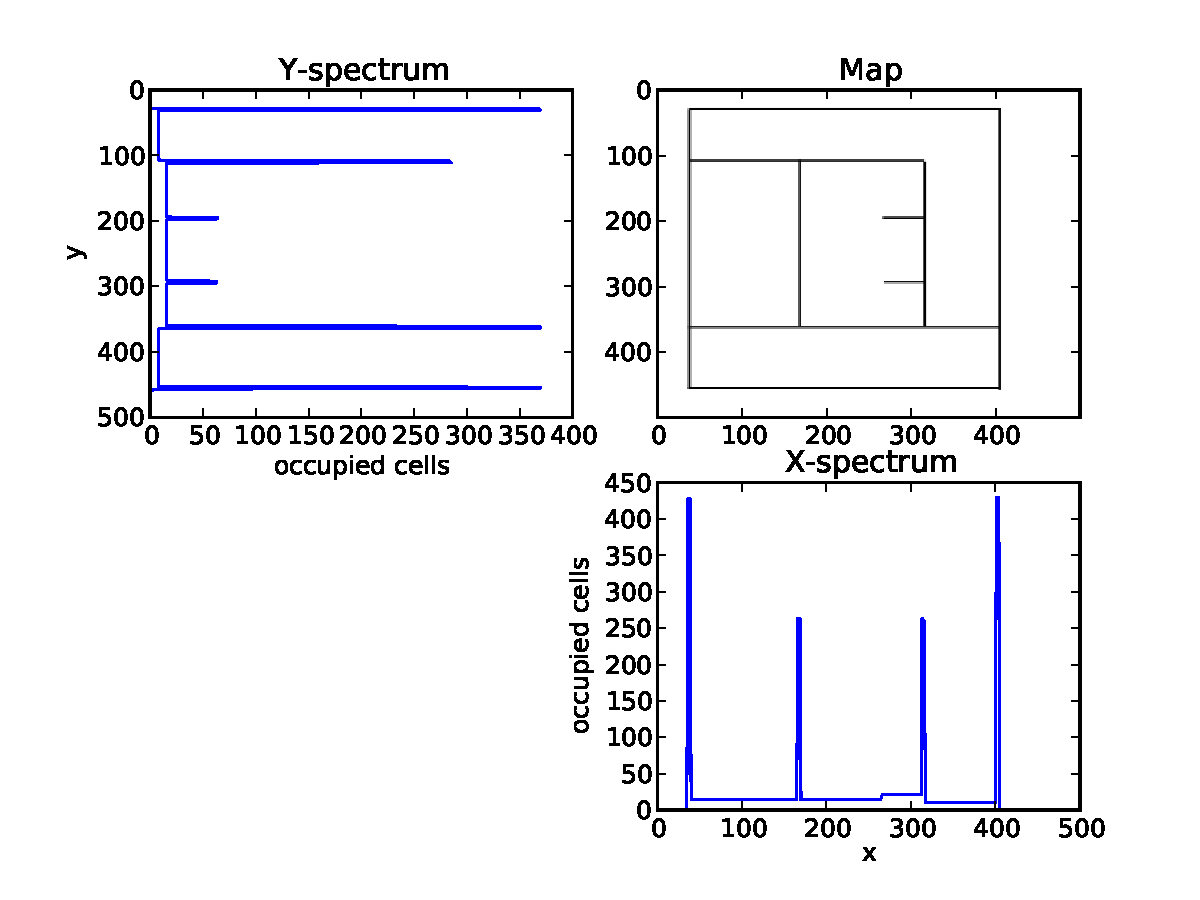
\includegraphics[width=\textwidth]{images/stitching/x_y_spectra.pdf}
	
	\caption{The original map (top right) with the y-spectrum (top left) and x-spectrum (bottom right).}
	\label{fig:x-y-spectra}
\end{figure}

Before the x- and y-spectra are taken of the image, care must be taken to align the image to the predominant direction $\phi$. In this way, the angular features of the environment (walls) show up as spikes in the spectrum. If the image is not aligned to the predominant direction $\phi$ the spectrum yields mostly noise, as can be seen in figure~\ref{fig:x-y-spectra-noise}.

\begin{figure}[ht]
	\centering
	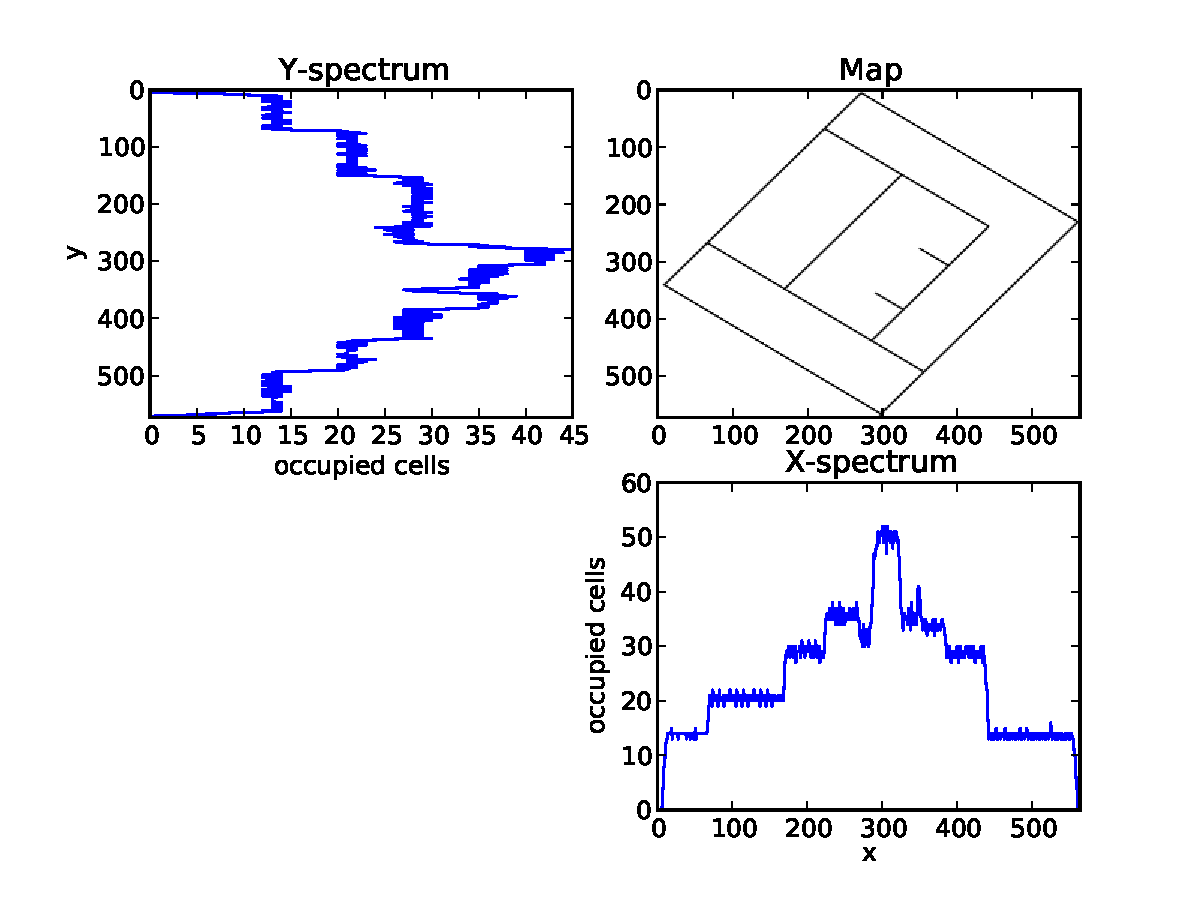
\includegraphics[width=\textwidth]{images/stitching/rooms-rotated-full-xy.pdf}
	\caption{The X- and Y-spectra of a map that is not aligned to the predominant direction $\phi$. Compare the spectra with those from figure \ref{fig:x-y-spectra}.}
	\label{fig:x-y-spectra-noise}
\end{figure}

Censi et~al.\ \cite{censi2005scan} propose a least-squares error optimization to find $\hat t$. Instead of taking a X-spectrum and Y-spectrum, the maps are rotated around many different angles and the spectra of those angles are cross-correlated. A least squares error solution is fit on the resulting optima. The X- and Y-spectrum method is a special case of this method; with only 2 constraint sets (one for the x-direction and one for y), the method yields an exact result for the two free parameters ($x, y$).

\section{Example}
Let's look at an example. We will examine more complicated cases in chapter~\ref{experiments}. In figure~\ref{fig:ex-rooms} you see again the image of the artificial map and a small piece which we will try and map onto the other. 

\begin{figure}[ht]
\centering
\subfigure[Full map]{
	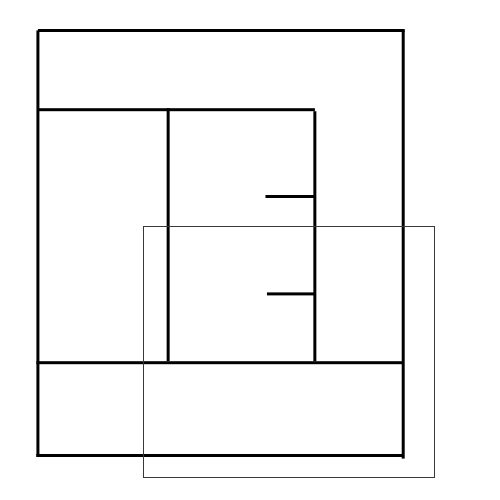
\includegraphics[width=0.4\textwidth]{images/stitching/rooms-full.png}
	\label{fig:ex-room-full}
}
\subfigure[Cutout]{
	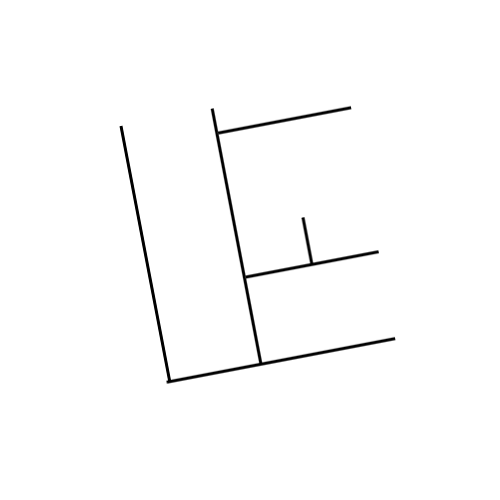
\includegraphics[width=0.4\textwidth]{images/stitching/rooms-partial.png}
	\label{fig:ex-room-cutout}
}
\caption{The map and a cutout that we want to match onto the map}
\label{fig:ex-rooms}
\end{figure}

The first step is to find candidate translations $\theta$. We do this by calculating the hough spectra and performing cross-correlation on them. See figure~\ref{fig:ex-cross-correlation}. The highest peak in the cross-correlation lies at $\theta_{1a} = 169\degree$, the second highest at $\theta_{2a} = 79\degree$. Because of the periodicity of the Hough spectrum there are also two dual-hypothesis: $\theta_{1b} = 180\degree+169\degree = 349\degree$ and $\theta_{2b} = 180\degree+79\degree = 259\degree$, respectively. Note that the first hypothesis and the second hypothesis lie $90\degree$ apart, which corresponds to the two main wall-directions in the image.

\begin{figure}[ht]
	\centering
	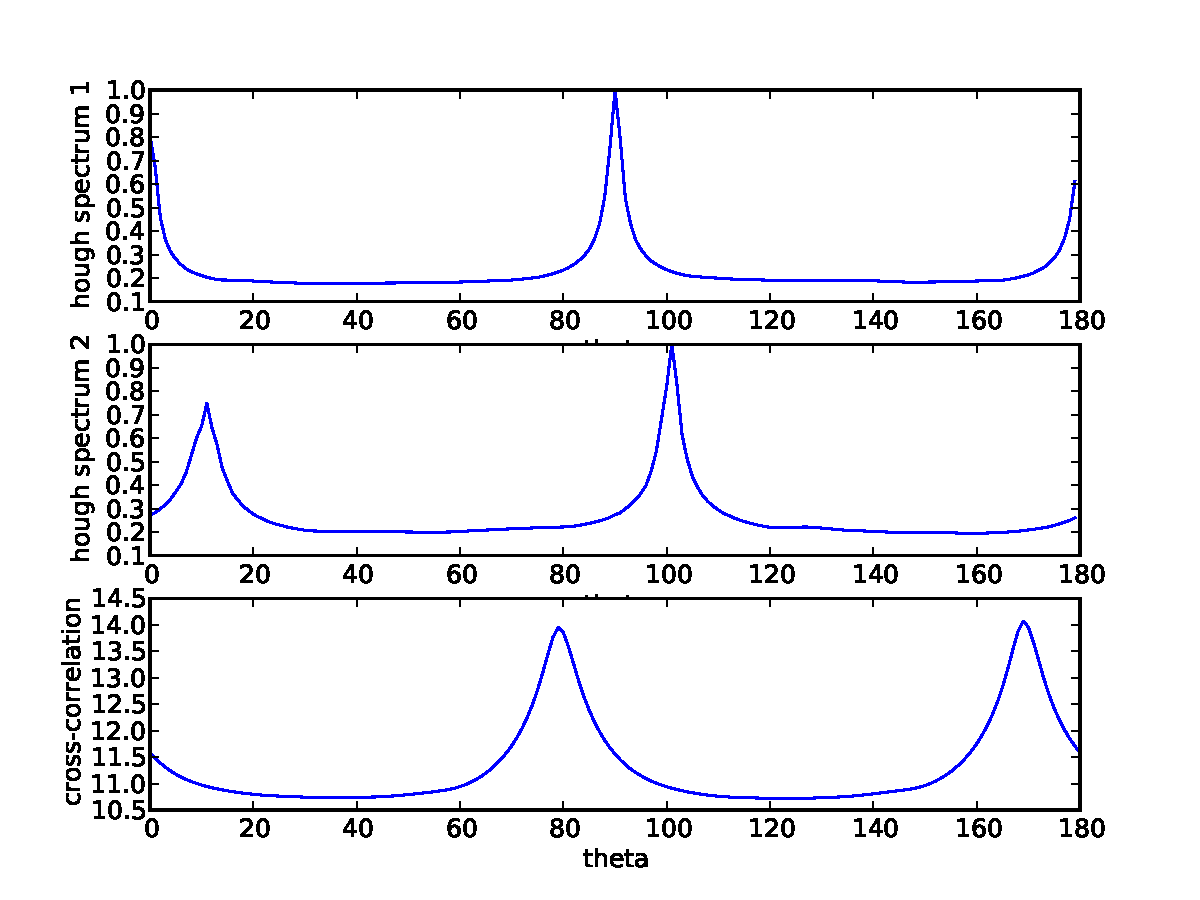
\includegraphics[width=\textwidth]{images/stitching/rooms-ex-match-theta.pdf}
	\caption{The Hough spectra of respectively figure~\ref{fig:ex-room-full} and \ref{fig:ex-room-cutout} and their cross-correlation.}
	\label{fig:ex-rooms-theta}
\end{figure}

As you can see in figure~\ref{fig:ex-rooms-theta}, the first image is not aligned with the predominant direction $\phi$: the highest peak in the hough spectrum lies at $90\degree$. Thus, we have to rotate it $90\degree$ counterclockwise before calculating the x- and y-spectra. Let's test the first hypothesis $\theta_{1a}$. We will rotate the cutout $169\degree + 90 \degree$ counterclockwise, according to the first hypothesis plus the predominant-direction correction. See figure~\ref{fig:ex-rooms-rotated}. In figure~\ref{fig:ex-rooms-spectra} you see the x-, y-spectra and their cross-correlations. 

\begin{figure}[ht]
	\centering
	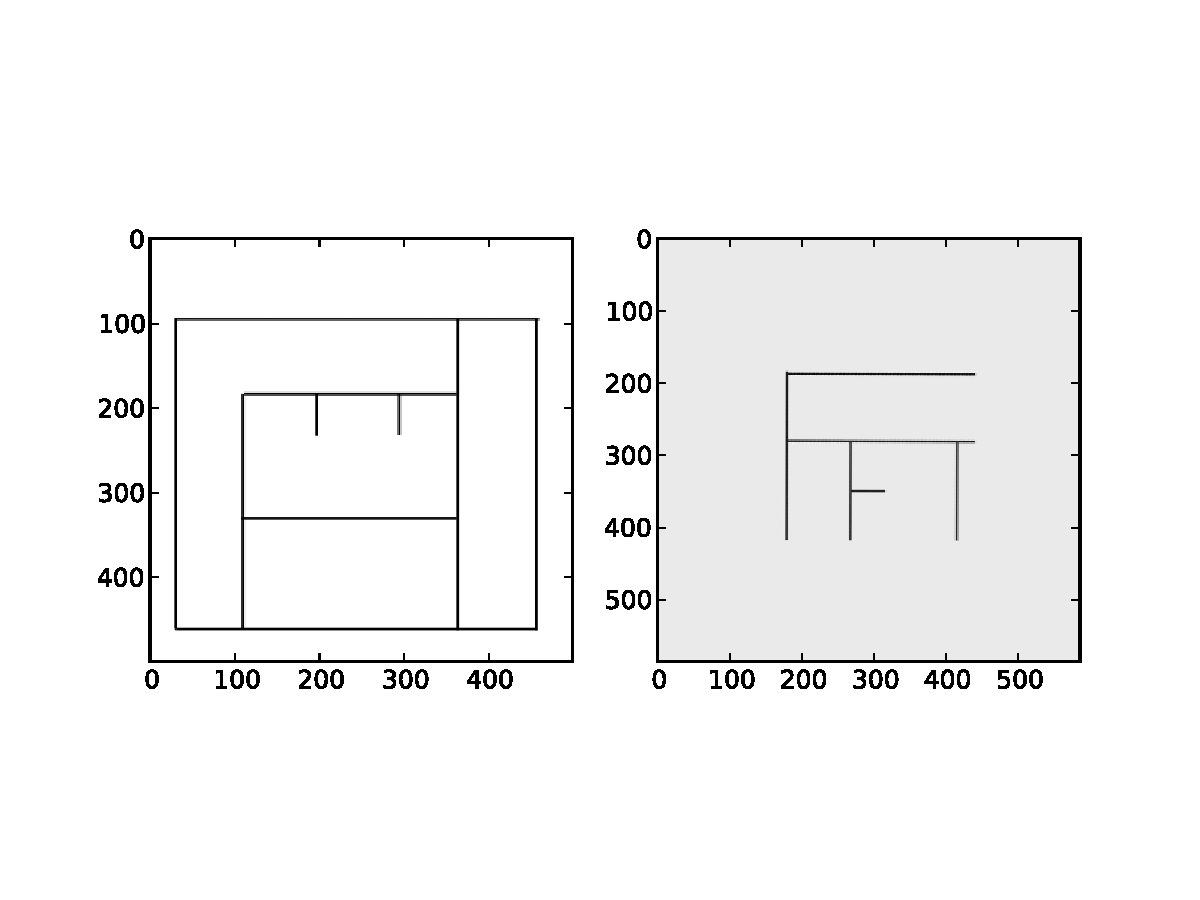
\includegraphics[width=\textwidth]{images/stitching/rooms-ex-rotated-crop.pdf}
	\caption{The images from figure~\ref{fig:ex-rooms} rotated along $\phi$ and $\phi + \theta_{1a}$, respectively}
	\label{fig:ex-rooms-rotated}
\end{figure}

\begin{figure}[ht]
	\centering
	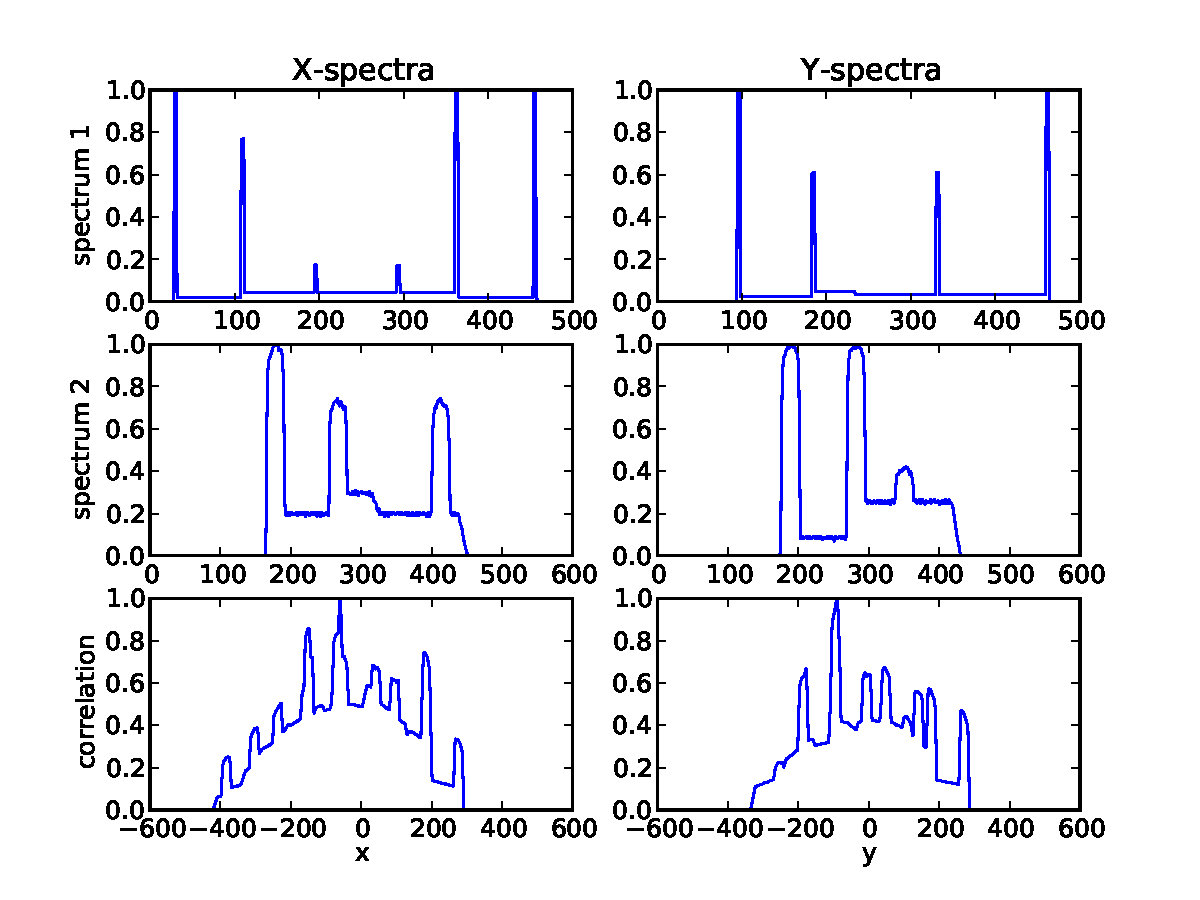
\includegraphics[width=\textwidth]{images/stitching/rooms-ex-xy-corr.pdf}
	\caption{The X- and Y-spectra and correlation of the images from figure~\ref{fig:ex-rooms-rotated}.}
	\label{fig:ex-rooms-spectra}
\end{figure}

The maxima in the X- and Y-spectra yield a translation estimate $\hat t = (-60, -89)$. In figure~\ref{fig:ex-rooms-result-1a} the result of the stitch is seen. The map is printed in blue, the cutout in pink. Astute readers will have noticed that the rotation estimate is $90\degree$ off, and the second hypothesis $\theta_{2}$ might yield a better result. They are right, as can be seen in figure~\ref{fig:ex-room-all-results} where the results for all $\theta$ hypothesis are shown.



\begin{figure}[ht]
\centering
\subfigure[$\theta_{1a}$]{
	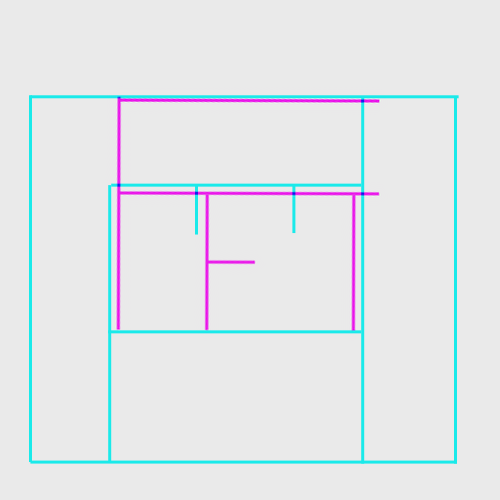
\includegraphics[width=0.3\textwidth]{images/stitching/rooms-ex-result-1a.png}
	\label{fig:ex-rooms-result-1a}
}
\subfigure[$\theta_{1b}$]{
	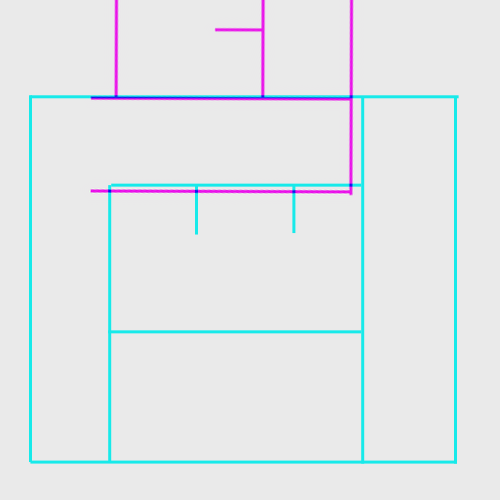
\includegraphics[width=0.3\textwidth]{images/stitching/rooms-ex-result-1b.png}
	\label{fig:ex-room-result-1b}
} \\
\subfigure[$\theta_{2a}$]{
	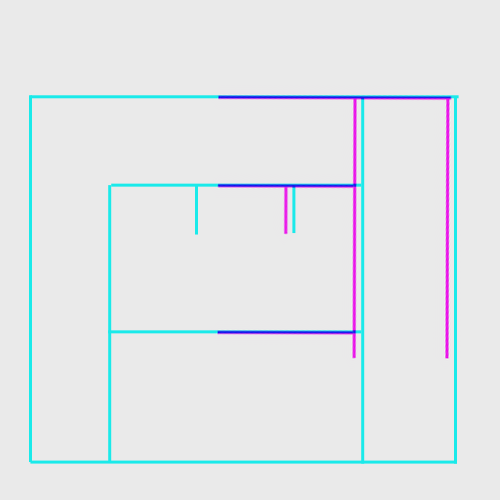
\includegraphics[width=0.3\textwidth]{images/stitching/rooms-ex-result-2a.png}
	\label{fig:ex-rooms-result-2a}
}
\subfigure[$\theta_{2b}$]{
	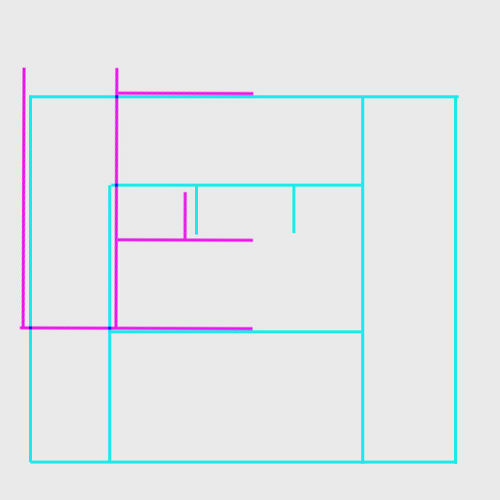
\includegraphics[width=0.3\textwidth]{images/stitching/rooms-ex-result-2b.png}
	\label{fig:ex-room-result-2b}
}
\caption{The results of map stitching according to all four $\theta$ hypothesis. Hypothesis $\theta_{2a}$ yields the correct result.}
\label{fig:ex-room-all-results}
\end{figure}